In this chapter we will go through the basic setup of the organization, how we work in the project as well as how we communicate within our project. 

\subsection{Roles}
After the applications for different roles were handed in to the project group, the members of the project decided who was going to be appointed to what specific role. Some of the roles applied for was decided not necessary for this type of project, which is why those applicants were assigned different roles. In the end, the company succeeded to appoint people to all the important positions in the company. 

\begin{figure}[hbt!]
\centering
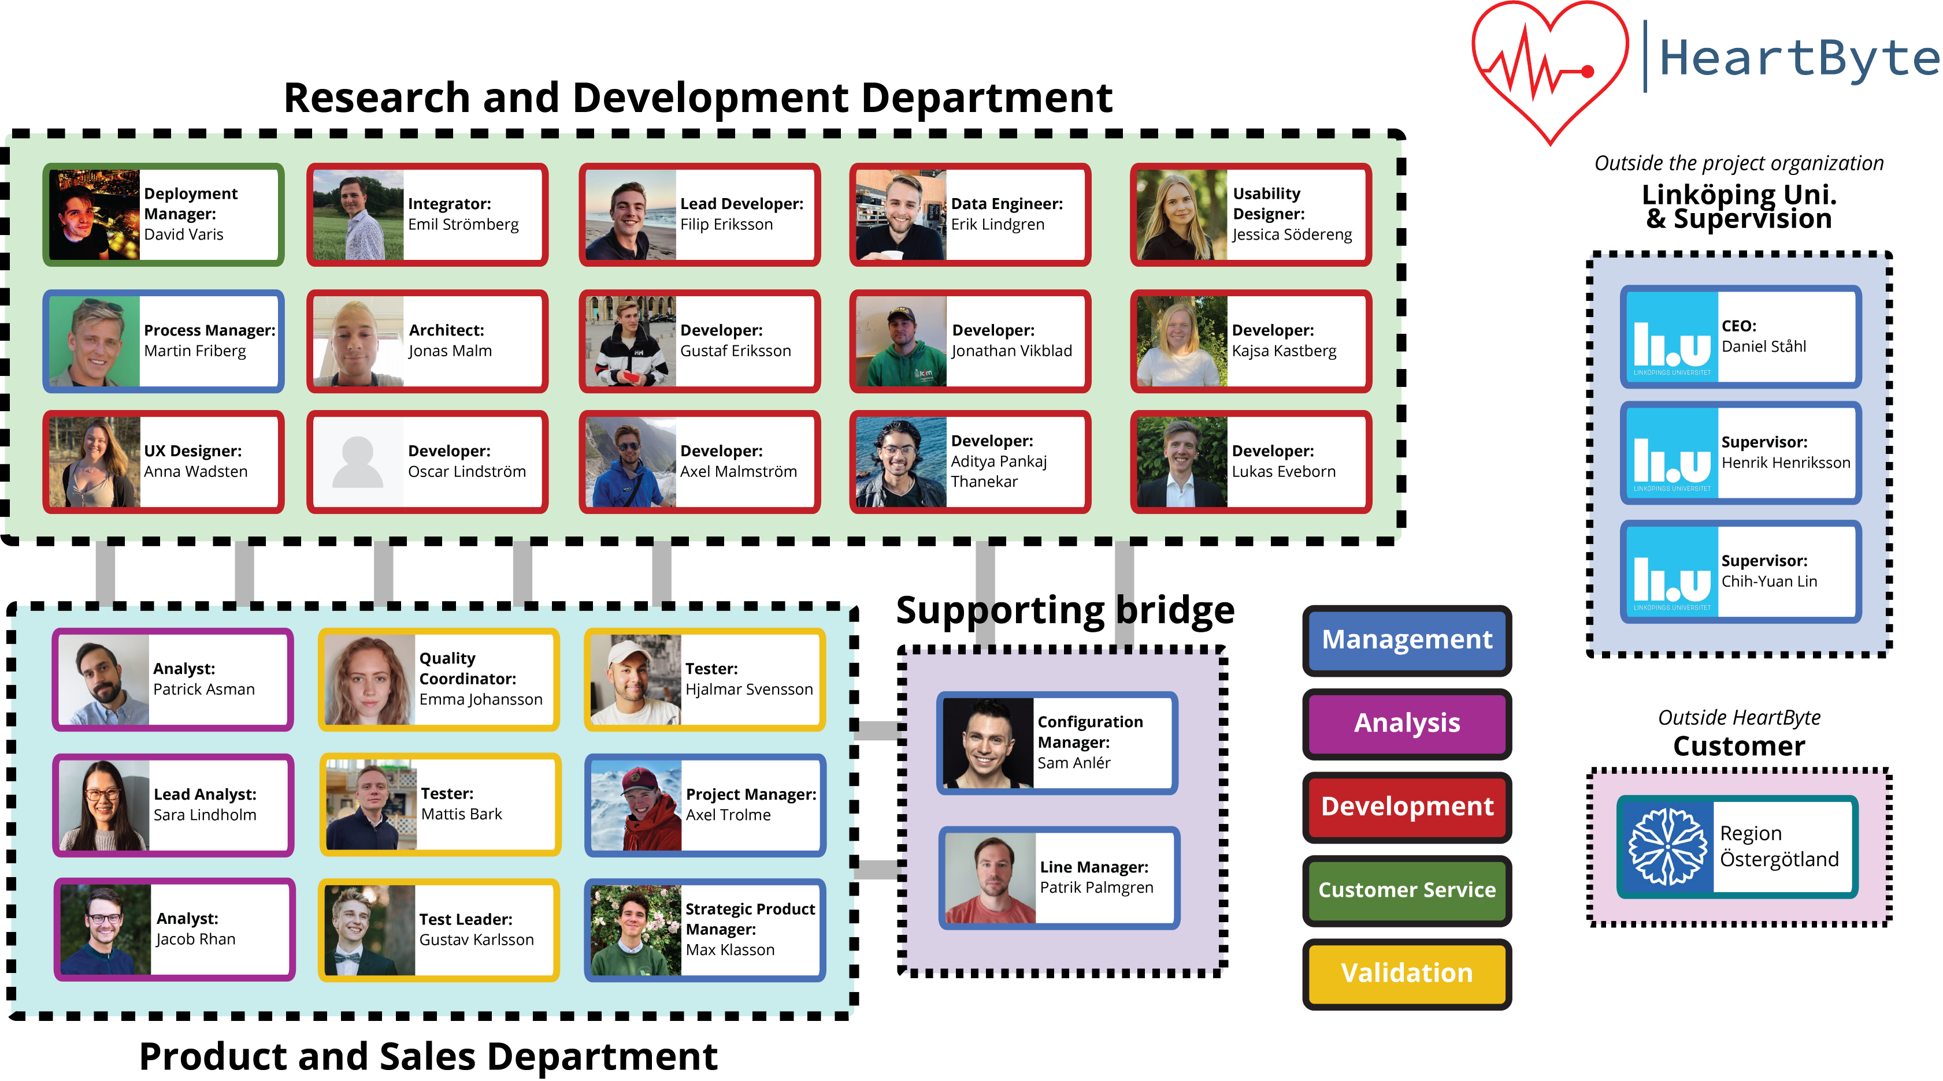
\includegraphics[width=\linewidth]{Pictures/Organization.png}
\caption{HeartByte project group}
\label{fig:company structure}
\end{figure}

The project group is divided into two major departments, the Research and Development department and the Product and Sales department. Within and across these groups there are also a number of smaller groups that are responsible for working with a certain task such as testing, developing, analyzing the system or managing the group.Cross-functional groups will be created in order to apply a broader knowledge when developing a certain feature or working with a certain task requiring knowledge from different departments. For example it is a good idea to include an analyst when developing a feature in order to assure that the quality and function of the feature is in line with what the software is supposed to achieve according the the applicable requirements. \\ 

The different roles within our organization all fills different purposes. The main goal is to create an organization where we're able to deliver the product ordered by our customer, on time and with the intended quality. In order to be able to do so, the organization has to be built up b a couple of different teams, see description below. 

\subsubsection{Management}
The main purpose for the management team is to coordinate the different tasks that has to be done in order to meet the goals for the project. Furthermore, the management team is responsible for coordinating the communication within the organization and to make sure that all the different sub teams has the information needed in order to pursue a certain task. The management team is built up by five different managers with different areas management questions to handle. Axel Trolme as the project manager is responsible for making sure that the project is on time and to deliver the information needed to the different parts of the organisation. Max Klasson as the strategic product manager is responsible for having the communication with our customer and to make sure that the information is correctly reflected in the requirements list as well as communicating with our development team. Patrik Palmgren as the line manager has become responsible for the safe keeping of documents and to make sure that all the living documents are up to date and with the quality needed. Sam Anlér as the configuration manager is responsible for keeping a continuous communication with all the team members and to make sure that the correct information is provided. Martin Friberg as the Process manager is responsible for mapping all the processes and to document them in the process plan. 

\subsubsection{Development}
The development team is responsible for writing the code of the product and to make detailed development decisions. 
\subsubsection{Validation}
\subsubsection{Customer Service}
\subsubsection{Analysis}

\subsection{Knowledge/skill}
The company management sent out a form to all the members of the company where the members were supposed to fill in what knowledge they have from before and what knowledge they are currently lacking. In this way, management is able to locate in what areas the skill and knowledge is high and in what areas we are lacking skill and knowledge. The languages chosen by our architect Jonas Malm for developing our Handle Many Platform is: React for front-end development and a combination of Flask and Python for the back-end development. Since React was not mapped in the knowledge and skill survey, the management makes the assumption after talking to most of the developers, that the knowledge within React is fairly limited. This fact has made the management produce a short term plan for introducing the new environment to the developers, where the first step is to watch the tutorial videos regarding react. In regards to further development the management outsources the major responsibility of sharing knowledge, acquiring a knowledge base and making the development of the project to the lead developer Filip Eriksson. 

\subsection{Training}
When working on the project, new skills has to be developed among the team members. In order to do so, different ways of training and education is provided. The sections below will give a brief description of how this is made. For more detailed information, please see the education plan document. 
\subsubsection{Workshops}
When development methods include new tools, we select someone responsible for the area who is supposed to gain a deeper understanding about the aforementioned tool. The person mentioned is then in charge of making sure that the rest of the team that is supposed to work with the tool gains the required knowledge about it. This is done via workshops online where the responsible person goes through the basics of the tool.  A workshop could also include different brainstorming activities, where the participants are to come up with ideas regarding risks, company name, requirements for the system or tools to use for a specific system. 

\subsubsection{Presentations}
The management produces presentations to give during CEO meetings to educate the team in what has been done during the week and what is to be done during the upcoming weeks. The management is also supposed to highlight what in the process that is the most critical to get done as soon as possible. The presentations might also be used to educate the team in processes and tools that makes the work more effective. Example of tools that this may include is GitLab, Microsoft Teams and different programming languages. The presentations could also focus more on education, for example how to handle documents and where to place them to be easily found once they are needed. The focus is to provide the team with the skills and information needed. To find more information regarding education, please see the education plan document. 

\subsubsection{Resource sharing}
Through sharing resources in Teams and GitLab the team tries to share the knowledge and progression within their work. This assures that the whole team gets to take part of each other’s knowledge and where they currently are in terms of progression. It also prevents two people from doing the same thing on two different ends. 

\subsection{Communication and reports}
Since the organization is fairly big with 26 members, we need to have structured ways in how we're handling communication throughout the team. The sections below will give a better insight in this process. 
\subsubsection{Group meetings and Discussions}
As stated previously in the report, the team is mainly separated into two departments. From these departments, cross-functional teams and teams where the whole group is working together on a specific task is created. The cross-functional teams makes it easier to share the information between the research and development department and the product and sales department as well as between the different specialized groups of analysts, testers, developers and management. Project group meetings are supposed to take place at least once every week where the CEO of the company as well as the entire project group is present. Alongside with these meetings other cross-functional meetings are to take place where the groups gets feedback from supervisors of the project. From the supervisors, the cross-functional teams can discuss problems, ideas and functionality of the software or other project related topics. 

\subsubsection{Communication directives}
The task specific groups reports mainly to the team leader of their group. Matters of importance are then to be communicated between different team leaders and management in order to lower the amount of group members that have to have direct communication with each other. This way of communicating also helps the project group and in particular the management to assure that knowledge that concerns parts of or the entire project group reaches the members that it concerns. Team leaders may also have direct contact with each other regarding a task that is specific to only their teams. When the cross-functional teams are set up for a specific task, the team members of the task is of course meant to have direct contact with each other, but if important matters arise, they are to be communicated to their team leaders who can forward the information to management. Management is then to produce a plan to circumvent or deal with the problem. 

\subsubsection{Reports}
In order to keep the investors, CEO and the customer satisfied and up to date with what is going on in the project, the team will announce weekly status reports. The status reports contains what the group has done during the last week, what is most crucial to be done during the upcoming week as well as what time each project member has put down into the project. This can also help the CEO keep track of the time spent in the project in order to not exceed the budget. There are also certain living documents that are to be produced in order for the entire team to stay updated about what the latest specifications are for the project. An updated version of the living documents are to be put in the general folder in the shared Microsoft Teams channel at the start of iterations 2-4. The updated documents are to be inspected by the management in order to assure quality of the documents. 
